\section{Explore} {
    Dalla pagina iniziale Home è possibile accedere alla pagina ``\textbf{Explore}'' cliccando sulla barra di navigazione il pulsante con tale scritta.

    La pagina contiene una lista di profili social che l'utente non segue, e gli vengono suggeriti in quanto sono i profili più virali, con maggior numero di followers.
    Infatti per ogni profilo social suggerito compare:
    \begin{itemize}
        \item Username: ovvero il suo nome utente;
        \item Followers: ovvero il numero di utenti della piattaforma \platform{} che seguono tale profilo social;
        \item Segui: un bottone che quando viene cliccato aggiunge il profilo social alla lista dei profili seguiti.
    \end{itemize}

    \begin{figure}[H]
        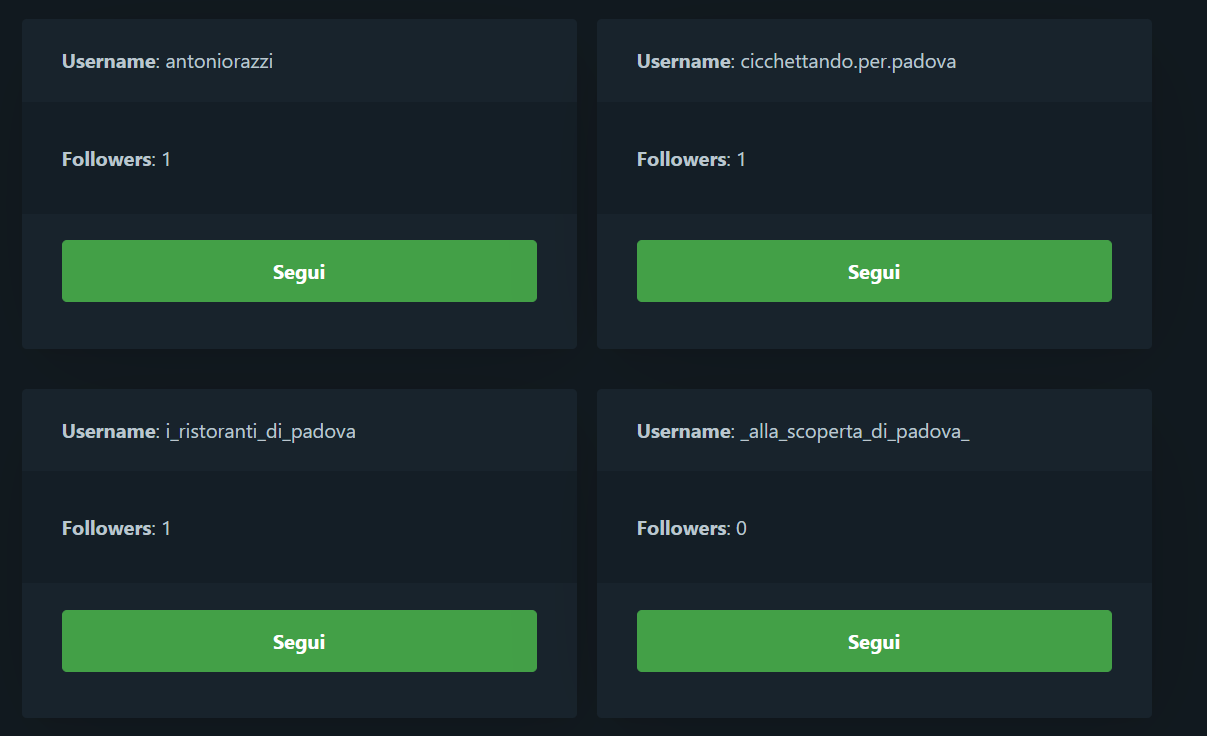
\includegraphics[width=12cm]{sezioni/images/explore.png}
        \centering
        \caption{Visualizzazione profili più popolari}
    \end{figure}
}   

